\documentclass{article} 
\usepackage{url, graphicx}
\usepackage[margin=1in]{geometry}
\usepackage{listings}

\title{Graph and Path Search Library Design Document}
\author{
Andrew Grant\\
\texttt{amg2215@columbia.edu}
\and 
Anton Igorevich \\
\texttt{ain2108@columbia.edu}
\and
 Somya Vasudevan \\
 \texttt{sv2500@columbia.edu}
}
\date{4/28/2017}

\begin{document}

\maketitle

\section{Introduction}
We've built a graph and path searching library, built in C++. The library is designed to make it really easy for users to use their own vertex and edge data structures and get going using graphs and running algorithms on them right away. Currently the library supports the following graphs: DG (directed graph), DAG (directed acyclic graph), DT (directed tree), Matrix(undirected). The idea is that users define their own vertex and edge data types, and then the library handles everything else under the hood. We also provide very generic path searching code that can be used in many domains. 

\section{Motivation}
Conceptually, a graph is made up of a bunch of vertices and edges. At a minimum there must be some way to distinguish between vertices, distinguish between edges, and define edges as made up of two vertices. Nonetheless, users often want to embed extra information in these ADTs. For example, a user may want a graph representing cities and the highways between them. The user may have a City class; cities must of course have some unique id (e.g. city name), but they may also have extra information such as population, GDP, etc. The same goes for edges; maybe a Road class is used, and the class also has miles, age of road etc. 
\par
We wanted to design a library that made it super easy for users to user their \emph{own} vertex and edge data types.
The philosophy of the library was that it should be really easy for users to be able to use their own vertex and edge data structures, and that the the library would handle everything else under the hood. In order to make it easy to use the library, we designed the library with minimal requirements when it came to the user defined vertex and edge types. 

\section{General Graph Design}
\subsection{Graph Data Types}
We provide the following graph types: DG (adjacency list), DAG (adjacency list), DT (adjacency list), and Matrix (undirected). All of these types are represented by simple structs. Each struct holds certain information about the graph it is representing. For example, the adjacency list structs will point to lists of vertices, while the matrix struct will point to some sort of matrix. An important member type of each struct is \texttt{graph\_type}. This member type is set to one of: \texttt{DAG, DG, DT, Matrix\_graph}. Concepts (described below) use this member type to determine what graph type is being used, and thus be able to determine, at compile type, which function to call. This is important as fundamentally there is no structural difference between a DT and DG; by using this member type we can have a function that works on a DT (and checks to make sure the tree structure invariant is maintained) and another function that works on a DG (and doesn't have to check that tree structure is maintained).

\subsection{User Defined Data Structures}
The library was designed so that users are able to design their own vertex and edge data structures. All that is required of the users is the following:
\begin{itemize}
\item Vertex and Edge must be comparable (that is they must implement the == operator for their types)
\item Vertex and Edge must be hashable
\item Edge must have two fields \texttt{v\_1} and \texttt{v\_2}, that are of the same type as the Vertex that they defined.
\item To use the path algorithms, Edge must have a cost field that is numeric. If the user does not define a cost, the library will automatically given an edge a cost of 1.
\item Vertex must have a \texttt{to\_string} function that returns a string representation of the vertex. 
\end{itemize}

\subsection{Wrappers}
Because minimal requirements are imposed on the user when it comes to his/her vertex and edge type, we needed to wrap the users data types in our own struct for certain bookkeeping reasons. Thus, under the hood the graph library stores each vertex in a \texttt{vertex\_wrapper} and each edge in a \texttt{edge\_wrapper}. Both wrappers also store a field of type \texttt{Value} which is a pair consisting of a string and an int. This lets the user set some sort of value for each vertex and/or edge, without their own data type knowing about such a value. Lastly, the wrapper also stores a unique id (of type int) that the user is again completely oblivious to. This id is generated by the graph library for internal bookkeeping (for example, it's used as the index when a matrix graph representation is used). The following image illustrates this.

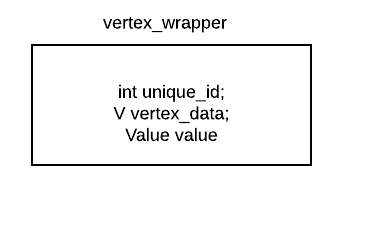
\includegraphics{vertexwrapper}

The idea is the same for the \texttt{edge\_wrapper}

\texttt{vertex\_data} points to the user provided vertex data. This \texttt{vertex\_wrapper} is the fundamental data type of our graph library. Whether a DAG, DG, DT or matrix graph representation is used, each vertex is stored in this struct. 

\subsection{Graph Interface}
Because all graphs are represented by structs, pretty much every graph library function requires such a graph struct as a formal argument. The remaining arguments are almost always one of the user defined vertex or edge. Thus, users do not need to know about wrappers at all. The wrappers are handled by the library. Furthermore, \texttt{shared\_ptr<>s} are required when using the API. That is, the library requires every formal argument to be of type \texttt{shared\_ptr<>} 
\par
Concepts allow us to use the same function name for different graph types. For example, there is a different function \texttt{add\_edge(G g, E e)} for each graph type.
\begin{lstlisting}
template<typename G, typename E>
requires Graph<G> && Edge_ptr<E>
bool add_edge(G g, E e)
{
	bool added_edge = add_edge_blindly_w_edge(g, e);
	return added_edge;
}

template<typename G, typename E>
requires DAG_Graph<G> && Edge_ptr<E>
bool add_edge(G g, E e)
{
	typedef typename G::element_type::vertex_type vertex_type;
	shared_ptr<vertex_type> tmp_v1 = make_shared<vertex_type>(e->v1);
	shared_ptr<vertex_type> tmp_v2 = make_shared<vertex_type>(e->v2);
	bool path_ex = path_exists(g, tmp_v2, tmp_v1);
	if (path_ex == true) {
		return false;
	} 
	bool added_edge = add_edge_blindly_w_edge(g, e);
	return added_edge;
}

template<typename G, typename E>
requires DT_Graph<G> && Edge_ptr<E>
bool add_edge(G g, E e)
{
	typedef typename G::element_type::vertex_type vertex_type;
	shared_ptr<vertex_type> tmp_v1 = make_shared<vertex_type>(e->v1);
	shared_ptr<vertex_type> tmp_v2 = make_shared<vertex_type>(e->v2);
	bool path_ex = path_exists(g, tmp_v2, tmp_v1);
	if (path_ex == true) {
		return false;
	}
	bool has_par = has_parent(g, tmp_v2);
	if (has_par == true) {
		return false;
	}
	bool added_edge = add_edge_blindly_w_edge(g, e);
	return added_edge;
}
\end{lstlisting}

\section{Adjacency List Design}
\subsection{}
DAG, DG and DT are are represented using adjacency lists. In order to implement an adjacency list, we actually created another data type to wrap \texttt{vertex\_wrapper}, which we call \texttt{vertex\_header}. The \texttt{vertex\_header} is the head of a vertex's adjacency list. Thus, the difference between a \texttt{vertex\_header} and \texttt{vertex\_wrapper}, is that the \texttt{vertex\_header} is the conceptual head of a vertex's adjacency list and points to a list of \texttt{vertex\_wrapper}.

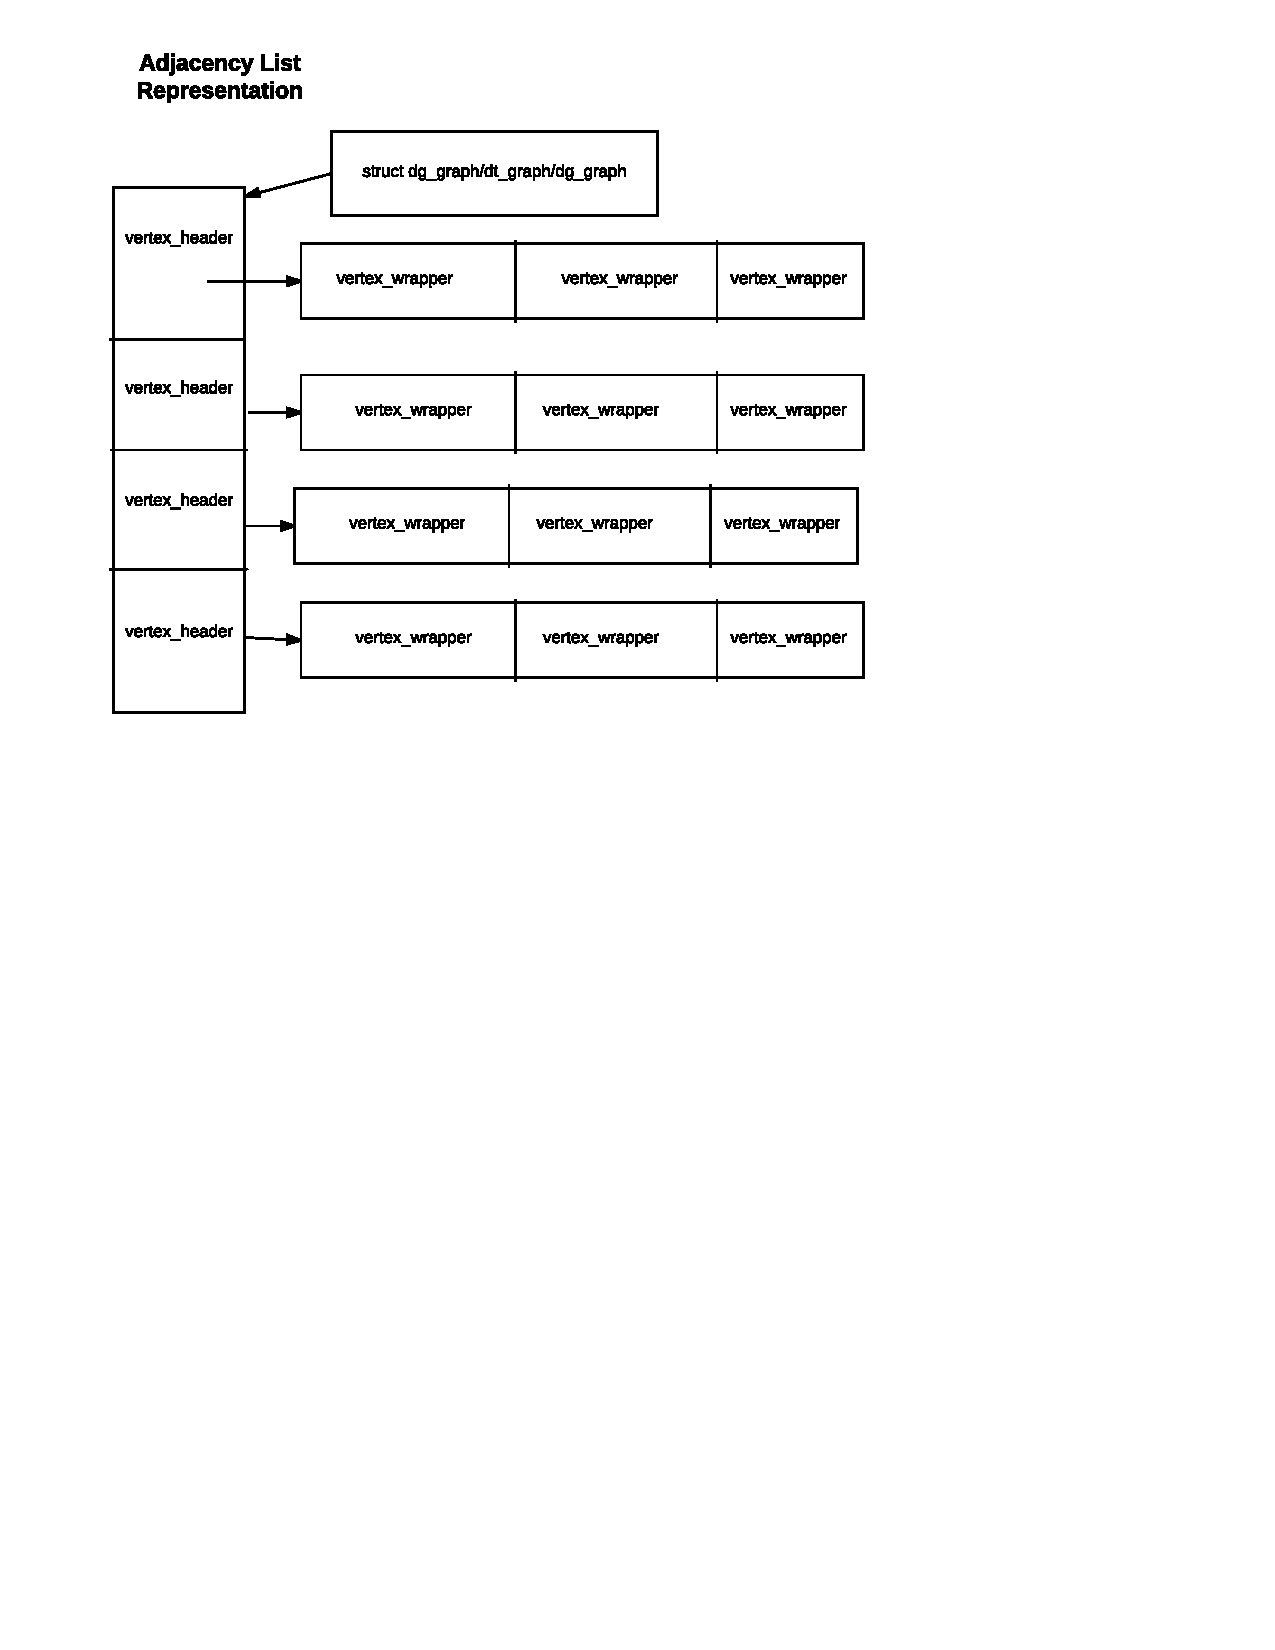
\includegraphics{al}

The image above shows the \texttt{vertex\_header} pointing to a list of \texttt{vertex\_wrapper}. \texttt{vertex\_header} actually also points to a list of \texttt{edge\_wrapper} too. 
\subsection{Data Structures}
The list of vertex headers is stored in a vector. The list of neighbors (aka \texttt{vertex\_wrapper} is also stored in a vector. The list of edges (aka \texttt{edge\_wrapper} is also stored in a vector).

\section{Matrix Design}
\subsection{}
As with the adjacency list representation, \texttt{vertex\_wrapper} is a fundamental data type to our matrix implementation. As emphasized, we wanted the user to be able to use his/her own vertex and edge types. In order to be as flexible as possible we did \emph{not} require the user to assign each vertex a unique integer id. Nonetheless, in order to use matrix graph representations we need some way to index each vertex into the matrix. We decided to use the internal id embedded in each \texttt{vertex\_wrapper} for this purpose. However, using this unique id wasn't enough. The whole point of using a matrix representation is the access efficiency; we needed some way to immediately map an incoming vertex to its unique id without iterating over \emph{all} vertices. Thus, to make the matrix representation work we maintain a hashmap pointing from a vertex to its \texttt{vertex\_wrapper}, which contains it's unique id. 

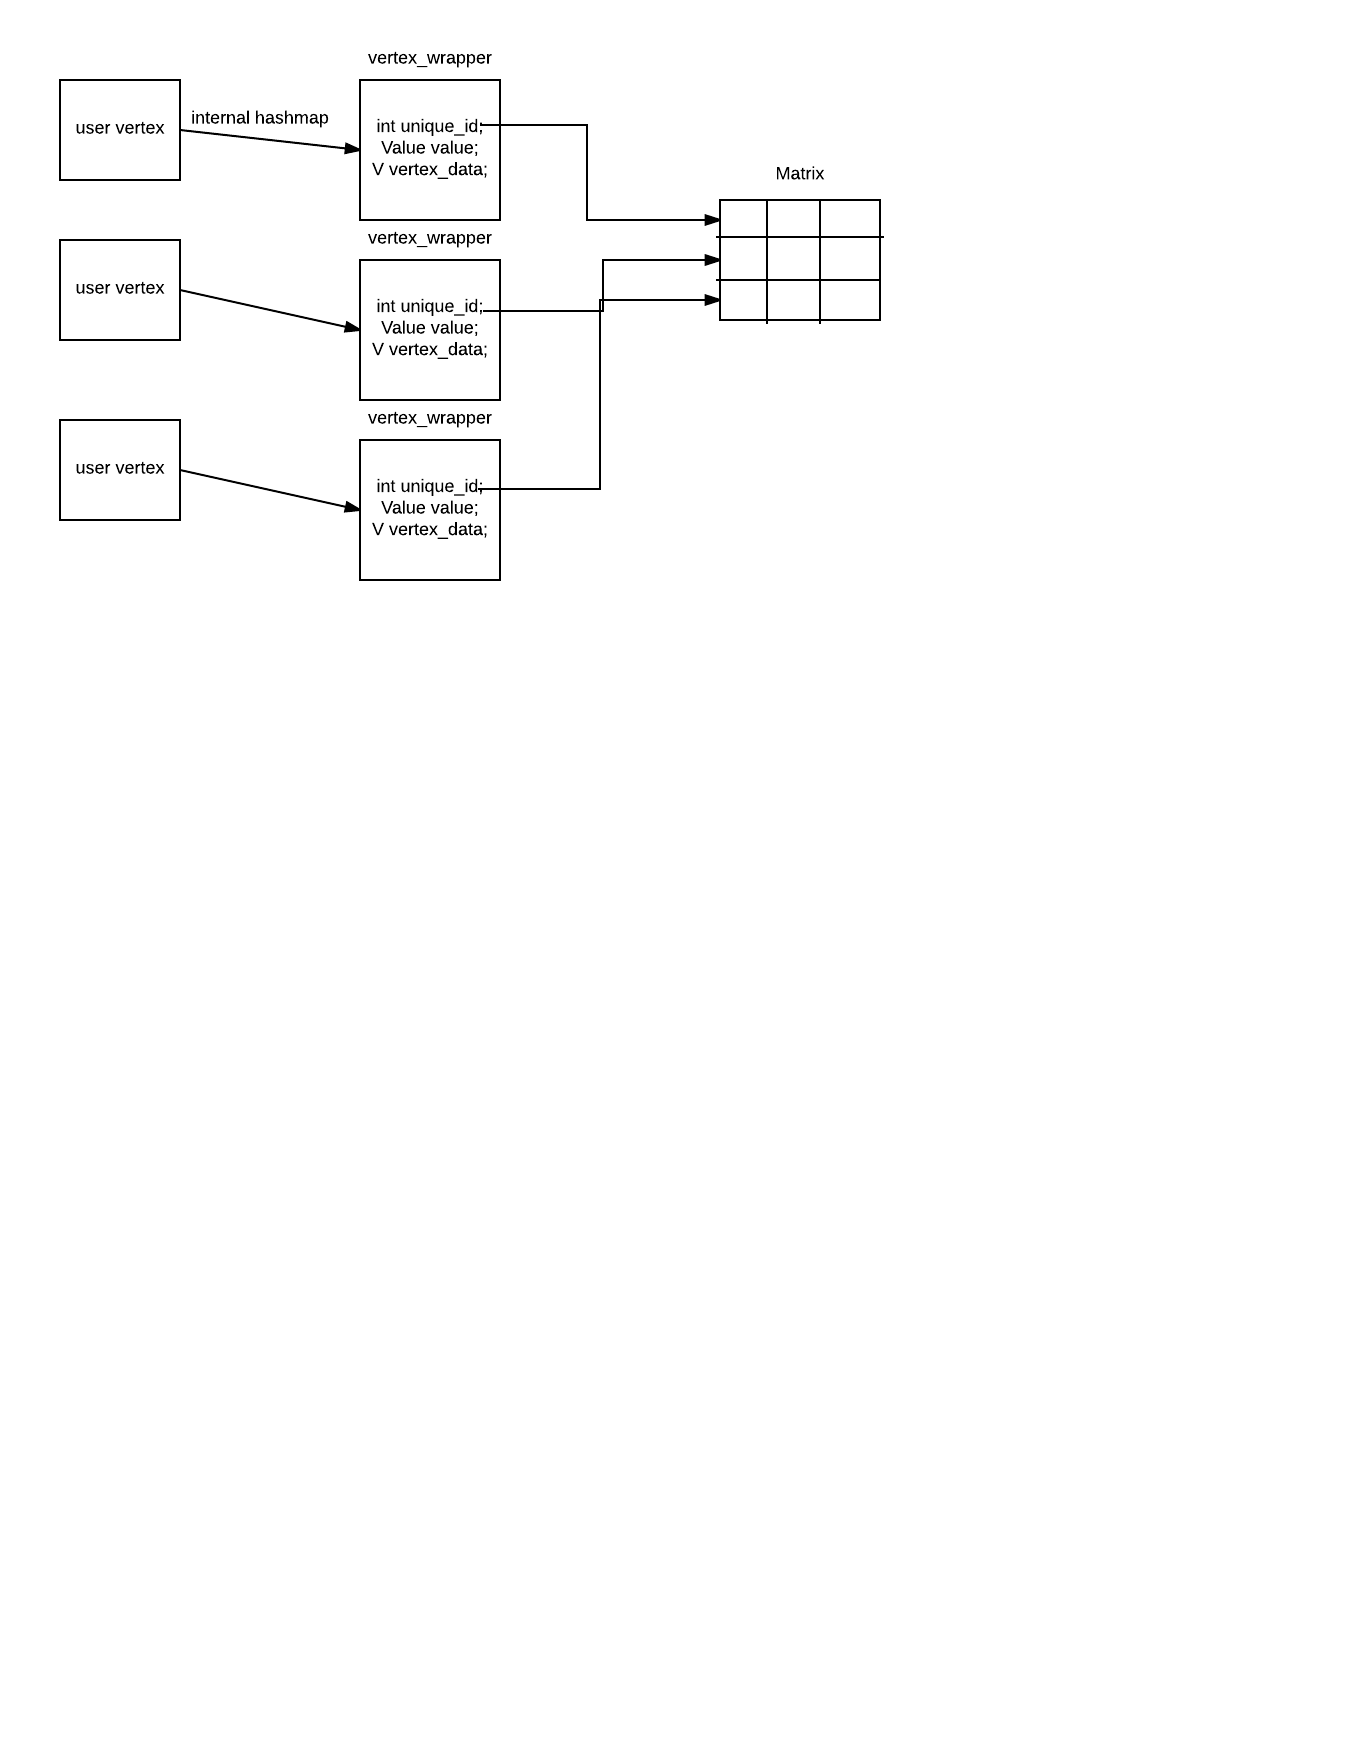
\includegraphics{matrix}

\subsection{Data Structures}
We use a vector of vectors to represent the matrix. Since the internal id is an int, the matrix is thus a vector of vector of ints. We also maintain a hashmap pointing from a vertex to its wrapper.

\section{Path Searching algorithms}
\subsection{Algorithms Supported}
We support the following path searching algorithms: 
\begin{itemize}
\item BFS
\item DFS
\item UCS
\item A*
\end{itemize}

\subsection{Implementation}
\subsubsection{User Defined State}
We designed the path algorithms such that they only require a ``start" state and ``goal" state, where ``state" is an abstract type. The user simply defines his/her own start and goal state, and the code handles the rest. Of course the semantics of path finding require that any given state must adhere to some requirements; we use concepts to enforce these:
\begin{itemize}
\item a state must be comparable
\item a state must be hashable
\item a state must have a \texttt{to\_string()} member function
\item a state must have a field called parent that is of type \texttt{shared\_ptr<state>}
\item a state must have a field called cost that is numeric
\item a state must have a member function called ``expand" that returns a vector of states
\item if A* is used, a member function called \texttt{heuristic\_func()} is required that returns a numeric type
\end{itemize}
As long as the user provides a type that adheres to these properties, any of our algorithms can be run

\subsubsection{Path Code}
We designed the path searching part of the library such that \emph{all} algorithms actually run on the same while loop. The function that eventually gets called accepts a few parameters that determine which algorithm gets run. For example, if we want to run DFS we send the path code a stack to be used as the frontier set. If we want to run BFS we send it a queue for the frontier set. Thus, all the different algorithms actually run on the same code; it's the inputs that decide which algorithm gets run. 
\par
Obviously we wouldn't want the user to know or worry about such details. Thus, the user simply calls \texttt{find\_path\_ast(s, g)}, and under the hood the library creates the appropriate frontier set and calls the generic code from there.

\subsubsection{Graph Library Integration}
The core graph library doesn't know anything about a ``start" state and a ``goal" state. A vertex is not the same thing as a state; for example, a vertex does not have the concept of a parent pointer. In order to use the path searching code, we therefore has to create state wrappers that integrated with the pre-existing graph data types. This made sure we could still use code described above, while also making sure the user did not have to worry about such transformations.

\section{Concepts}
\subsection{What are concepts?}
Concepts are essentially compile time predicates. That is, they are requirements on the types that are passed into functions. If an argument doesn't satisfy the concept, the compiler will immediately report an error. This makes debugging much easier when using templates. Without concepts, debugging can be very tricky when using templates, as it's often late in the compilation process that the compiler realizes a type is no good. As a result error messages can be extremely long, making dubugging tricky. 
\subsection{Library Usage}
In terms of this library, the idea is that user defined vertices and edges must satisfy certain properties; concepts are used to enforce these. For example, an Edge must point to two vertices; an Edge must be comparable; a Vertex must have a unique identifier. Perhaps more importantly, we use concepts to support function overloading. The names of the functions that work on different graph types are all the same; thus the user can call the same function whether he or she is working with a matrix or adjacency list. Concepts determine which function should be called at \emph{compile} time, not runtime. 

\subsection{References}
\begin{itemize}
\item Concepts reference: \url{http://www.stroustrup.com/good_concepts.pdf}
\item The complete project is located at \url{https://github.com/andyg7/Graph-Library}.
\item The core graph library code is located at \url{https://github.com/andyg7/Graph-Library/src}
\end{itemize}

\end{document} 